\section{Kirchhoff approximation}
\label{Sec4:Kirchhoffs}
The exterior Helmholtz problem is given by
\begin{alignat}{3}
	\nabla^2 p + k^2 p &= 0 	&&\text{in}\quad \Omega^+,\label{Eq4:HelmholtzEqn}\\
	\partial_n p &= g						&&\text{on}\quad \Gamma,\label{Eq4:HelmholtzEqnNeumannCond}\\
	\pderiv{p}{r}-\imag k p &= o\left(r^{-1}\right)\quad &&\text{with}\quad r=|\vec{x}|\label{Eq4:sommerfeldCond}
\end{alignat}
where the Sommerfeld condition in~\Cref{Eq4:sommerfeldCond} restricts the field uniformly in $\hat{\vec{x}}=\frac{\vec{x}}{r}$, such that no waves originate from infinity.

By Kirchhoff's integral theorem we have (cf.~\cite[Theorem 2.21]{Chandler_Wilde2012nab})
\begin{equation}\label{Eq4:KirchhoffIntegral}
	p(\vec{x}) = \int_{\Gamma}\left[ p(\vec{y})\pderiv{\Phi_k(\vec{x},\vec{y})}{n(\vec{y})} - \Phi_k(\vec{x},\vec{y})\pderiv{p(\vec{y})}{n(\vec{y})}\right]\idiff \Gamma(\vec{y})
\end{equation}
where $\vec{y}$ is a point on the surface $\Gamma$, $\vec{n}$ lies on $\Gamma$ pointing ``into'' $\Omega^+$ at $\vec{y}$ and $\Phi_k$ is the free space Green's function for the Helmholtz equation in \Cref{Eq4:HelmholtzEqn} given (in 3D) by
\begin{equation}\label{Eq4:FreeSpaceGrensFunction}
	\Phi_k(\vec{x},\vec{y}) = \frac{\euler^{\imag kR}}{4\PI R},\quad\text{where}\quad R = |\vec{x} - \vec{y}|.
\end{equation}
The derivative of Green's function is given by
\begin{equation*}
	\pderiv{\Phi_k(\vec{x},\vec{y})}{n(\vec{y})} = \frac{\Phi_k(\vec{x},\vec{y})}{R}(\imag kR-1)\pderiv{R}{n(\vec{y})},\quad\text{where}\quad\pderiv{R}{n(\vec{y})} = -\frac{(\vec{x}-\vec{y})\cdot\vec{n}(\vec{y})}{R}.
\end{equation*}
Moreover, for an incident wave $p_{\mathrm{inc}}$ satisfying the Helmholtz equation we have (using \cite[Theorem 2.20]{Chandler_Wilde2012nab})
\begin{equation*}
	\int_{\Gamma}\left[ p_{\mathrm{inc}}(\vec{y})\pderiv{\Phi_k(\vec{x},\vec{y})}{n(\vec{y})} - \Phi_k(\vec{x},\vec{y})\pderiv{p_{\mathrm{inc}}(\vec{y})}{n(\vec{y})}\right]\idiff \Gamma(\vec{y}) = 0.
\end{equation*}
Thus, we can write \Cref{Eq4:KirchhoffIntegral} in terms of the total pressure $p_{\mathrm{tot}} = p + p_{\mathrm{inc}}$
\begin{equation}
	p(\vec{x}) = \int_{\Gamma}\left[ p_{\mathrm{tot}}(\vec{y})\pderiv{\Phi_k(\vec{x},\vec{y})}{n(\vec{y})} - \Phi_k(\vec{x},\vec{y})\pderiv{p_{\mathrm{tot}}(\vec{y})}{n(\vec{y})}\right]\idiff \Gamma(\vec{y})
\end{equation}
For rigid scattering with $\partial_n p_{\mathrm{tot}} = 0$ we therefore have
\begin{equation}\label{Eq4:farfieldRigid}
	p(\vec{x}) = \int_{\Gamma}p_{\mathrm{tot}}(\vec{y})\pderiv{\Phi_k(\vec{x},\vec{y})}{n(\vec{y})} \idiff \Gamma(\vec{y})
\end{equation}
The \textit{far field pattern} for the scattered pressure $p$, is defined by
\begin{equation}\label{Eq4:farfield}
	p_0(\hat{\vec{x}}) =  \lim_{r\to\infty} r \euler^{-\imag k r}p(r\hat{\vec{x}}),
\end{equation}
with $r = |\vec{x}|$ and $\hat{\vec{x}} = \vec{x}/|\vec{x}|$. Using the limits
\begin{equation}\label{Eq4:Phi_k_limits}
\begin{aligned}
	&\lim_{r\to\infty} r\euler^{-\imag k r}\Phi_k(r\hat{\vec{x}},\vec{y}) = \frac{1}{4\PI}\euler^{-\imag k \hat{\vec{x}}\cdot\vec{y}}\\
	&\lim_{r\to\infty} r\euler^{-\imag k r}\pderiv{\Phi_k(r\hat{\vec{x}},\vec{y})}{n(\vec{y})} = -\frac{\imag k}{4\PI}\euler^{-\imag k \hat{\vec{x}}\cdot\vec{y}}\hat{\vec{x}}\cdot\vec{n}(\vec{y})
\end{aligned}	
\end{equation}
the formula in \Cref{Eq4:KirchhoffIntegral} simplifies in the far field to (cf.~\cite[p. 32]{Ihlenburg1998fea})
\begin{equation}\label{Eq4:KirchhoffIntegralFarField}
	p_0(\hat{\vec{x}}) = -\frac{1}{4\PI}\int_{\Gamma}\left[ \imag k p(\vec{y})\hat{\vec{x}}\cdot\vec{n}(\vec{y}) + \pderiv{p(\vec{y})}{n(\vec{y})}\right]\euler^{-\imag k \hat{\vec{x}}\cdot\vec{y}}\idiff \Gamma(\vec{y}).
\end{equation}
For rigid scattering this is simplified to (from \Cref{Eq4:farfieldRigid})
\begin{equation}\label{Eq4:KirchhoffIntegralFarField2}
	p_0(\hat{\vec{x}}) = -\frac{\imag k}{4\PI}\int_{\Gamma} p_{\mathrm{tot}}(\vec{y})\hat{\vec{x}}\cdot\vec{n}(\vec{y}) \euler^{-\imag k \hat{\vec{x}}\cdot\vec{y}}\idiff \Gamma(\vec{y}).
\end{equation}
From the far field pattern, the \textit{target strength}, $\TS$, can be computed. It is defined by
\begin{equation}\label{Eq4:TS}
	\TS = 20\log_{10}\left(\frac{|p_0(\hat{\vec{x}})|}{|P_{\mathrm{inc}}|}\right)
\end{equation}
where $P_{\mathrm{inc}}$ is the amplitude of the incident wave at the geometric center of the scatterer (i.e. the origin). Since the amplitude of the scattered pressure is proportional to the amplitude of the incident wave (due to the linearity of the Helmholtz equation), $\TS$ is independent of $P_{\mathrm{inc}}$.

Kirchoff's diffraction formula is derived by assuming the values of $p$ and $\partial_n p$ to be known at the boundary~\cite{Fawcett2001moh}. The value for the pressure $p$ at the boundary $\Gamma$ can be modeled by physical optics approximation~\cite[p. 147]{Chandler_Wilde2012nab}. In this case, we have
\begin{equation*}
	p_{\mathrm{tot}} = \begin{cases} 2p_{\mathrm{inc}} & \text{on illuminated sides}\\
		0 & \text{on sides in shadow}.
		\end{cases}
\end{equation*}
By considering plane waves 
\begin{equation}\label{Eq4:PlaneWave}
	p_{\mathrm{inc}} = P_{\mathrm{inc}}\euler^{\imag k\vec{d}_{\mathrm{s}}\cdot \vec{x}}
\end{equation}
and defining $\Gamma_{\mathrm{i}}$ as the illuminated sides of $\Gamma$, \Cref{Eq4:KirchhoffIntegralFarField2} is then reduced to
\begin{equation}\label{Eq4:bistatic}
	p_0(\hat{\vec{x}}) \approx -\frac{\imag kP_{\mathrm{inc}}}{2\PI}\int_{\Gamma_{\mathrm{i}}} \hat{\vec{x}}\cdot\vec{n}(\vec{y}) \euler^{\imag k (\vec{d}_{\mathrm{s}} - \hat{\vec{x}})\cdot\vec{y}}\idiff \Gamma(\vec{y}).
\end{equation}
For monostatic scattering we have $\vec{d}_{\mathrm{s}} =- \hat{\vec{x}}$, such that
\begin{equation}\label{Eq4:monostatic}
	p_0(\hat{\vec{x}}) \approx -\frac{\imag kP_{\mathrm{inc}}}{2\PI}\int_{\Gamma_{\mathrm{i}}} \hat{\vec{x}}\cdot\vec{n}(\vec{y}) \euler^{-2\imag k \hat{\vec{x}}\cdot\vec{y}}\idiff \Gamma(\vec{y}).
\end{equation}
In~\Cref{Fig4:BeTSSiresults} we illustrate the impact the convexity of a geometry has on two of the BeTSSi models~\cite{Nolte2014bib} visualized in~\Cref{Fig4:BeTSSiModels}. The reference solutions are computed by the ASIGA\footnote{The ASIGA (Acoustic Scattering with IsoGeometric Analysis) library can be found at \href{https://github.com/Zetison/ASIGA}{https://github.com/Zetison/ASIGA}.} library.
\begin{figure}
	\centering
	\begin{subfigure}{0.7\textwidth}
		\centering
		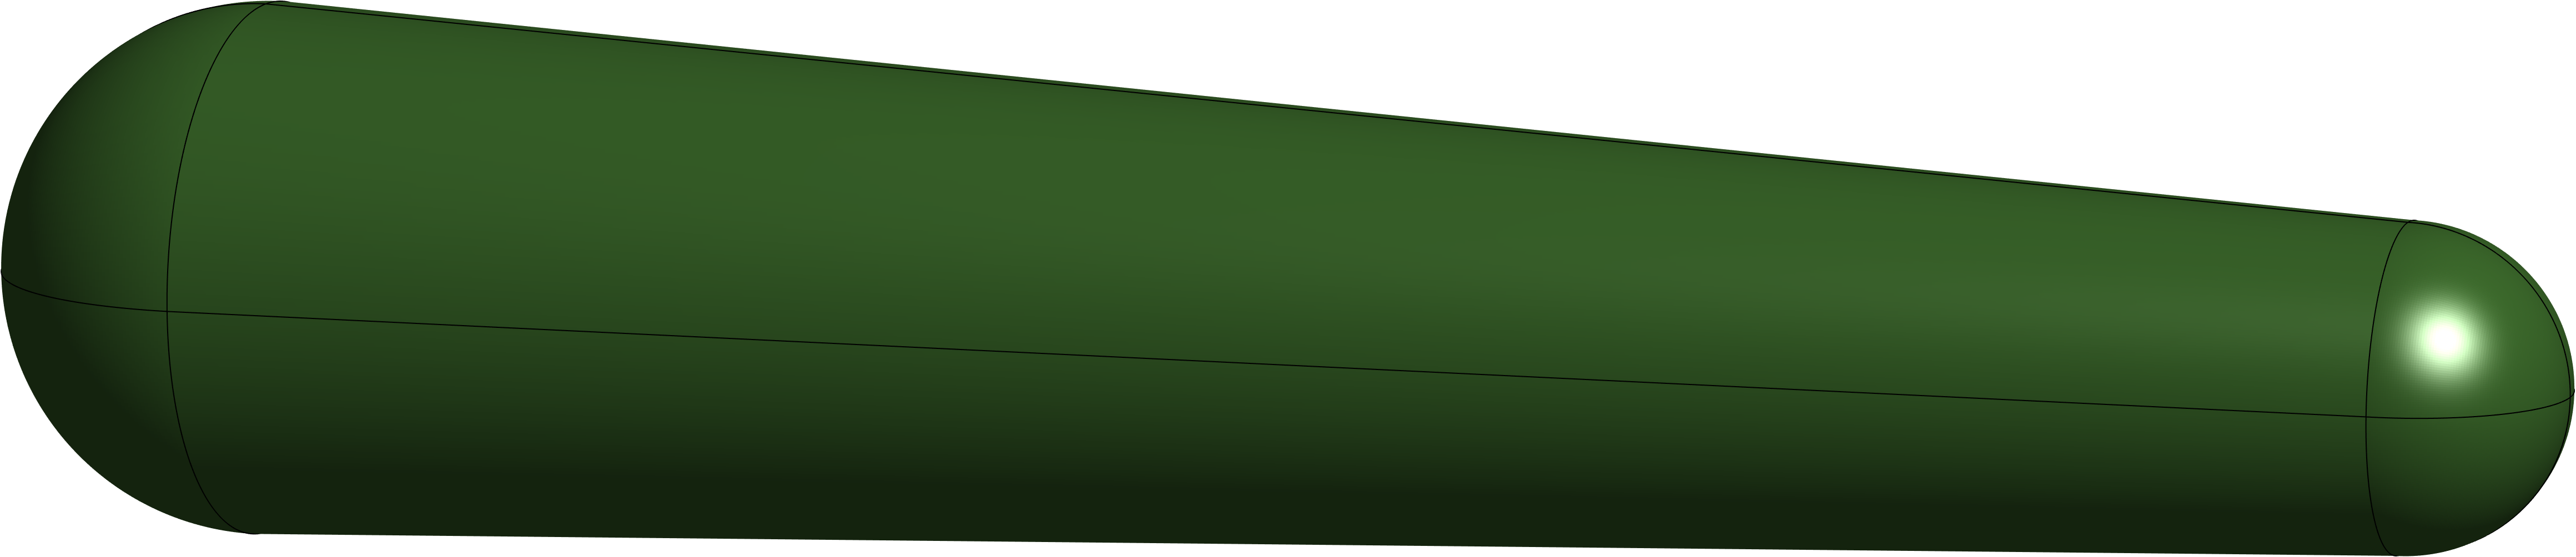
\includegraphics[width=0.9447\textwidth]{M3} % width = 0.6613/0.7
		\caption{The BeTSSi model 3}
	\end{subfigure}%
	\begin{subfigure}{0.3\textwidth}
		\centering
		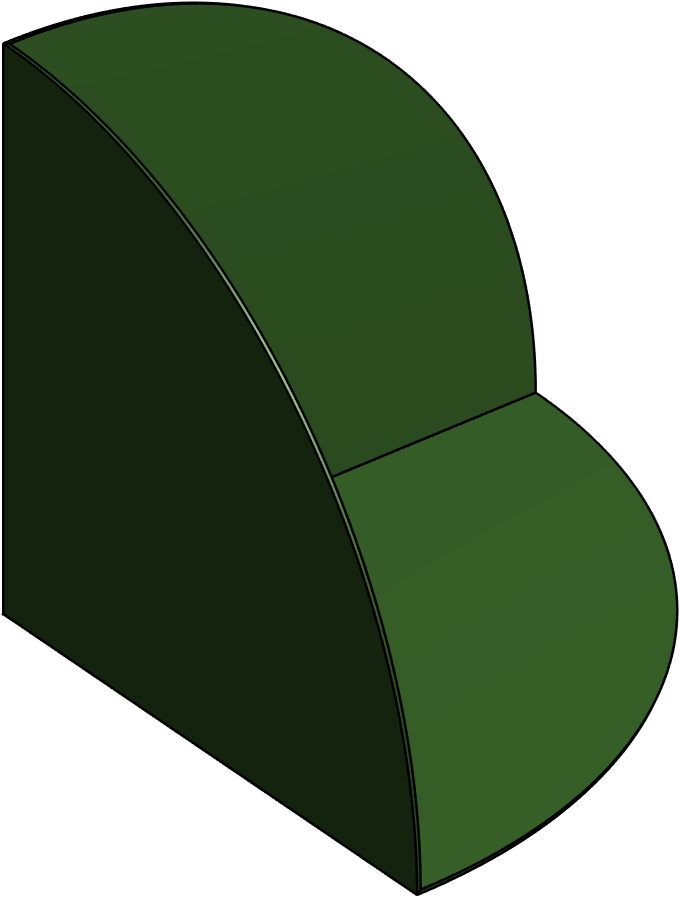
\includegraphics[width=0.4\textwidth]{BeTSSi_M4}
		\caption{The BeTSSi model 4}
	\end{subfigure}
	\par\bigskip
	\par\bigskip
	\begin{subfigure}{\textwidth}
		\centering
		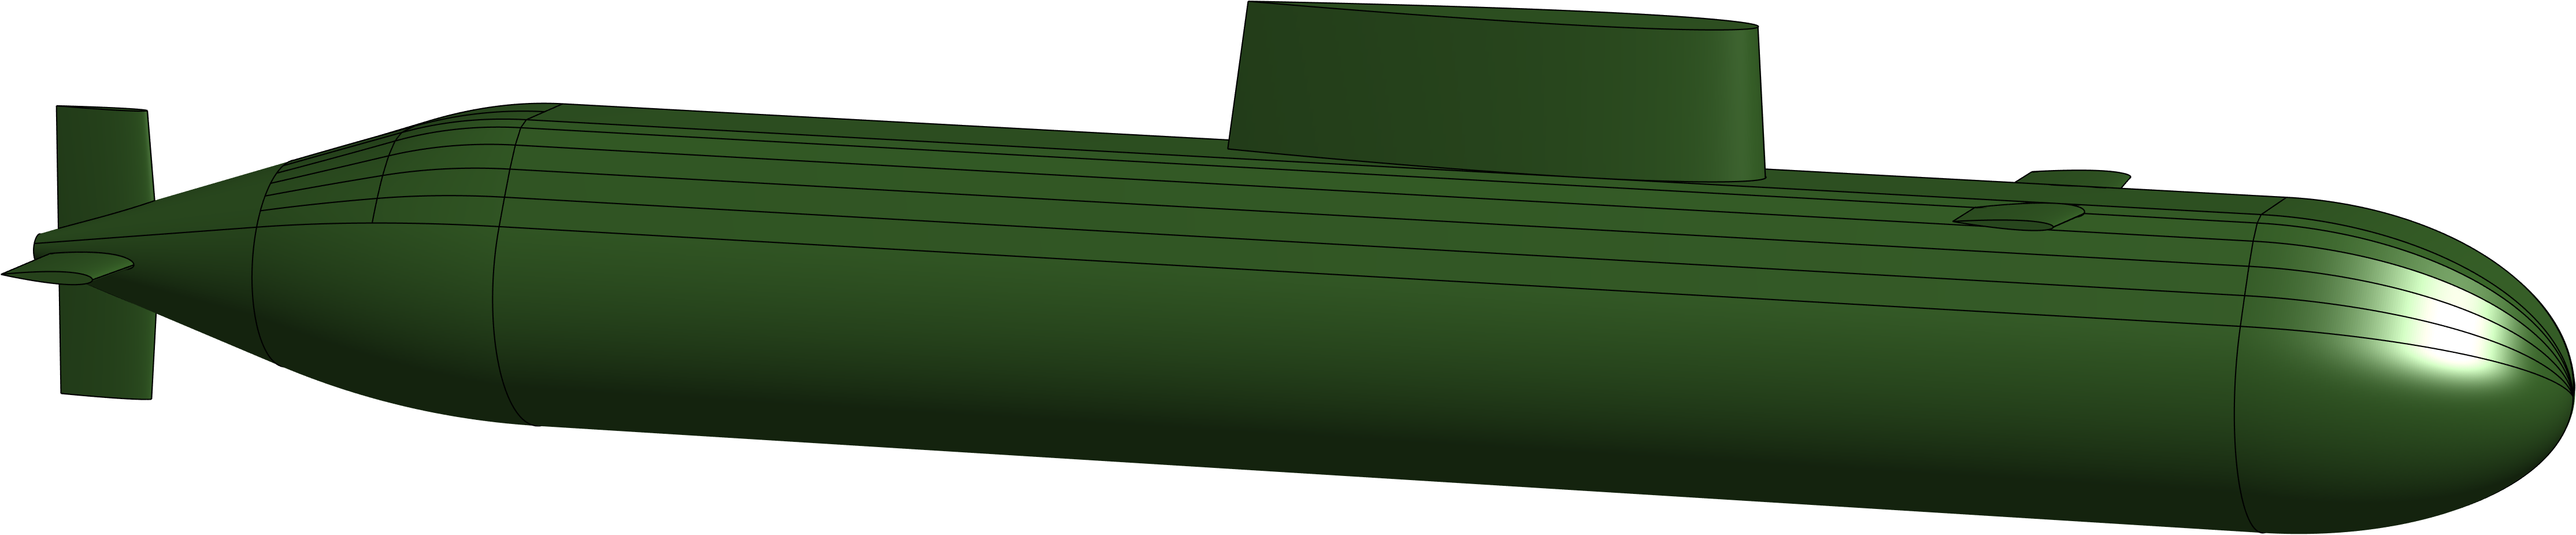
\includegraphics[width=\textwidth]{CAD}
		\caption{The BeTSSi submarine}
	\end{subfigure}
	\caption{The BeTSSi model 3 is described and analyzed in~\cite{Venas2015iao} and the BeTSSi submarine is described and analyzed in~\cite{Venas2019ibe}.}
	\label{Fig4:BeTSSiModels}
\end{figure}
The BeTSSi model 3 is nearly convex while the BeTSSi submarine is not. Despite this, good results are obtained for the BeTSSi submarine considering the simplicity of the Kirchhoff approximation method. The BEM simulation on the BeTSSi submarine was computed with \num{59488} elements with basis functions of $6^{\mathrm{th}}$ degree (resulting in \num{124113} degrees of freedom) with the Burton-Miller formulation. The simulation used \num{126650} seconds, and the Kirchhoff diffraction theory (KDT) simulation (with GL quadrature on IGA mesh) uses only \num{60} seconds on the same IGA mesh. This is reasonable since the complexity of a BEM solver is at least $\bigoh(n_{\mathrm{el}}^2)$ whereas the complexity of the KDT solver is only $\bigoh(n_{\mathrm{el}})$ assuming a given number of elements are needed for a given frequency and accuracy. Due to the exponential decay of the error in the numerical integration using Gauss--Legendre quadrature far less elements are needed for the KDT simulation compared to finite/boundary element methods (with algebraic convergence rates). The KDT simulation on only 3718 elements using $(\check{p}+1)^2=49$ GL points per element yields visually indistinguishable results for the BeTSSi submarine simulation with a computational timing of only a few seconds (not shown in~\Cref{Fig4:BeTSSiresults}).
\begin{figure}
	\centering
	\begin{subfigure}{\textwidth}
		\centering
		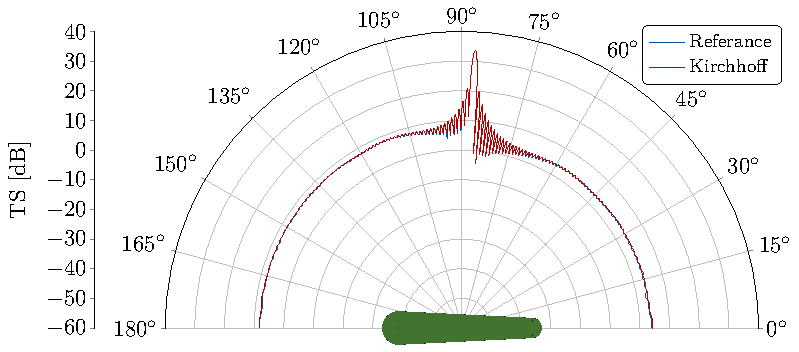
\includegraphics[width=\textwidth]{M3_MS}
		\caption{The BeTSSi model 3}
	\end{subfigure}
	\par\bigskip
	\par\bigskip
	\begin{subfigure}{\textwidth}
		\centering
		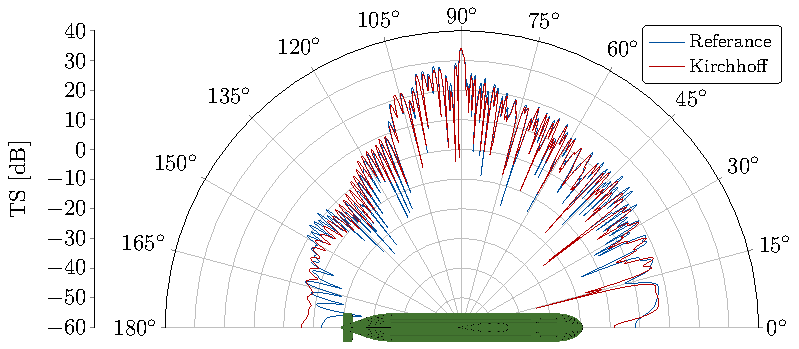
\includegraphics[width=\textwidth]{BCA_MS}
		\caption{The BeTSSi submarine}
	\end{subfigure}
	\caption{\textbf{Rigid scattering on BeTSSi models}: Comparison of the monostatic target strength (\Cref{Eq4:TS}) for the Kirchhoff approximation (\Cref{Eq4:exactHelmholtz}) and IGABEM reference solutions. The Kirchhoff approximation is obtained by classical Gauss-Legendre integration. This benchmark is one of the BeTSSi test cases with elevation angle $\beta_{\mathrm{s}}=\ang{0}$ and frequency $f=\SI{1}{kHz}$.}
	\label{Fig4:BeTSSiresults}
\end{figure}

For the BeTSSi model 4 the results deviate much more as can be seen in~\Cref{Fig4:BeTSSi_M4results}. This model is a corner reflector which yields high TS for aspect angles that ``sees'' this corner (i.e. $\alpha,\beta\in(0,\ang{90})$). Since Kirchhoff approximation does not handle multiple reflections, this domain yields particularly large discrepancies. 
\begin{figure}
	\centering
	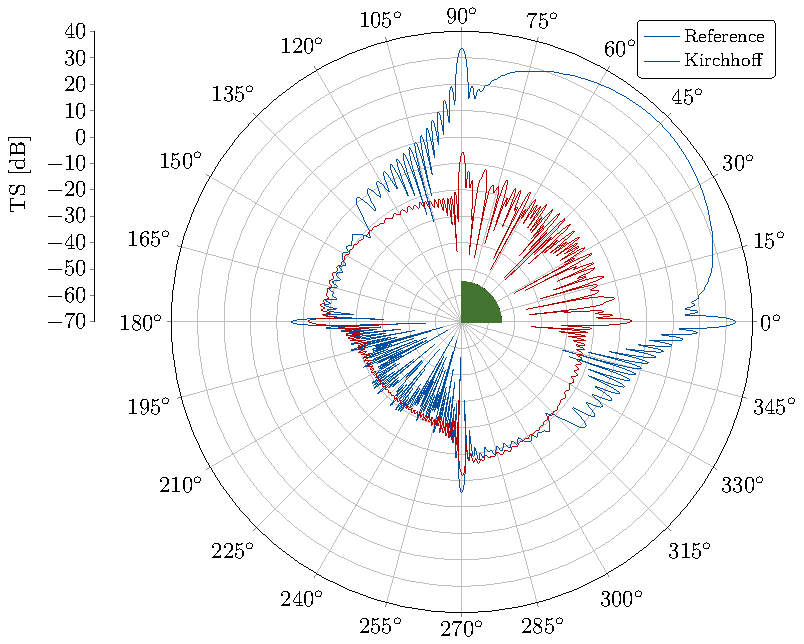
\includegraphics[width=\textwidth]{M4_MS}
	\caption{\textbf{Rigid scattering on BeTSSi model 4}: Comparison of the monostatic target strength (\Cref{Eq4:TS}) for the Kirchhoff approximation (\Cref{Eq4:exactHelmholtz}) and a IGABEM reference solution. The Kirchhoff approximation is obtained by classical Gauss-Legendre integration. This benchmark is one of the BeTSSi test cases with elevation angle $\beta_{\mathrm{s}}=\ang{30}$ and frequency $f=\SI{10}{kHz}$.}
	\label{Fig4:BeTSSi_M4results}
\end{figure}

If the domain $\Gamma_{\mathrm{i}}$ is polygonal and the boundary of $\Gamma_{\mathrm{i}}$ lies on polygonal edges, the integrals in \Cref{Eq4:bistatic,Eq4:monostatic} can be exactly evaluated by subdividing each polygon into triangles and using barycentric coordinates. On each triangle $\Gamma_{\mathrm{i},n}$ the barycentric coordinates are given by
\begin{equation}\label{Eq4:y_xi}
	\vec{y} = \vec{y}(\xi_1,\xi_2) = (\vec{P}_{n,1}-\vec{P}_{n,3})\xi_1 + (\vec{P}_{n,2}-\vec{P}_{n,3})\xi_2 + \vec{P}_{n,3}
\end{equation}
where $\vec{P}_i$ are the corners of the triangle. Then the integral in \Cref{Eq4:monostatic} may be written as
\begin{align}
	p_0(\hat{\vec{x}}) &\approx -\frac{\imag kP_{\mathrm{inc}}}{\PI}\sum_{n=1}^N|\Gamma_{\mathrm{i},n}|\int_0^1\int_0^{1-\xi_1} \hat{\vec{x}}\cdot\vec{n}_n\euler^{-2\imag k \hat{\vec{x}}\cdot\vec{y}}\idiff \xi_2\idiff\xi_1\nonumber \\
	&= -\frac{\imag kP_{\mathrm{inc}}}{\PI}\sum_{n=1}^N|\Gamma_{\mathrm{i},n}|\hat{\vec{x}}\cdot\vec{n}_n\int_0^1\int_0^{1-\xi_1} \euler^{D_{n,0}+D_{n,1}\xi_1+D_{n,2}\xi_2}\idiff \xi_2\idiff\xi_1\nonumber \\\label{Eq4:polygonalApprox}
	&= -\frac{\imag kP_{\mathrm{inc}}}{\PI}\sum_{n=1}^N|\Gamma_{\mathrm{i},n}|\hat{\vec{x}}\cdot\vec{n}_ng(D_{n,1},D_{n,2})\euler^{D_{n,0}}
\end{align}
with
\begin{align*}
	g(D_{n,1},D_{n,2}) &= \int_0^1\int_0^{1-\xi_1} \euler^{D_{n,1}\xi_1+D_{n,2}\xi_2}\idiff \xi_2\idiff\xi_1 \\
	&= \frac{D_{n,1}(1-\euler^{D_{n,2}})+D_{n,2}(\euler^{D_{n,1}}-1)}{D_{n,1}D_{n,2}(D_{n,1}-D_{n,2})}
\end{align*}
\begin{align*}
	D_{n,0} &= -2\imag k\hat{\vec{x}}\cdot \vec{P}_{n,3}\\
	D_{n,1} &= -2\imag k\hat{\vec{x}}\cdot (\vec{P}_{n,1} - \vec{P}_{n,3})\\
	D_{n,2} &= -2\imag k\hat{\vec{x}}\cdot (\vec{P}_{n,2} - \vec{P}_{n,3}).
\end{align*}
Note that
\begin{align*}
	\lim_{D_{n,1}\to 0} g(D_{n,1},D_{n,2}) = -\frac{1}{D_{n,2}^2}\left(1+D_{n,2}-\euler^{D_{n,2}}\right),\\
	\lim_{D_{n,2}\to 0} g(D_{n,1},D_{n,2}) = -\frac{1}{D_{n,1}^2}\left(1+D_{n,1}-\euler^{D_{n,1}}\right),\\
	\lim_{D_{n,1},D_{n,2}\to 0} g(D_{n,1},D_{n,2}) = \frac{1}{2},\\
	\lim_{D_{n,1}\to D_{n,2}} g(D_{n,1},D_{n,2}) = \frac{1}{D_{n,2}^2}\left(1-\euler^{D_{n,2}}+D_{n,2}\euler^{D_{n,2}}\right).
\end{align*}
If $\Gamma_{\mathrm{i}}$ does not lie on polygonal edges, some geometric errors are introduced which goes to zero when $h_{\mathrm{max}}\to 0$. Usually, $\Gamma$ is not only represented by polygonal surfaces. However, using a tessellation of the model where this approach can be employed is the most common way of using Kirchhoff approximation.